\documentclass[a4paper,11pt]{article}
\usepackage[american]{babel}
\usepackage[utf8]{inputenc}
\usepackage{geometry}
\usepackage{float}
\usepackage{booktabs}  
\usepackage{graphicx}
\usepackage{listings}
\usepackage{amsmath}
\lstset{%
backgroundcolor=\color{cyan!10},
basicstyle=\ttfamily,
numbers=left,numberstyle=\scriptsize
}

\usepackage[wby]{callouts}

\title{Convolutional Sparse Coding With Different TV Regularizations }
\author{Fa Long}

\begin{document}

\maketitle

\section{Introduction}~

The idea of parsimony, which is about representing some phenomenon with as few variables as possible. is being used in many different areas. such as statistics, signal processing and computer vision. In signal processing, signals is approximated  in a sparse linear combination of prototype called dictionary elements. People choose dictionary elements in many different ways, for example, some people use wavelets basis as dictionary atoms, since wavelets have interesting properties to be localized both in the space and frequency domains. so it's very suitable to multi-resolution analysis of signals, like digital image signals.\\

In 1996, Olshausen and Field proposed a very significantly different approach which, instead of using a fixed dictionary,  they proposed to 'learn' a dictionary from training data~\cite{DBLP:journals/corr/MairalBP14}. and they proved that dictionary learning can easily reveal underlying structure of nature image patches, after that, dictionary learning had been used in a huge amounts of applications.\\

The patch wised sparse coding is appropriate for processing natural image patches \cite{4011956}\cite{1640847}. A natural extension to full images instead of patches is called “convolutional sparse coding”. It consists of linearly decomposing an image by using small dictionary elements placed at all possible locations in the image. Such a principle was described early by Zhu et al. [2005] without concrete application. It has been revisited recently, and has been shown useful for various recognition tasks\cite{DBLP:journals/corr/MairalBP14}. However, convolutional sparse representation is inferior to the original patch-wise convolutional sparse coding, and the biggest problem for this type of method is the cost of computation, that is the reason why it hasn't been used until recently, a very fast and efficient way to solve this problem has been found by using ADMM structure\cite{7308045}. To boost up the performance of convolutional sparse representation, several regularizer has been combined with traditional convolutional sparse representation, Total Variation(TV) on coefficient map is one of those, There are experiments show that 2D TV with convolutional sparse representation can promote the performance of convolutional sparse representation. Instead of 2D TV, We introduced a new type of TV which not only evaluate the differences along horizontal and vertical axis of the coefficient map, but also evaluate the gradient between each coefficient maps.
\\

During my independent study, I studied an efficient way to solve convolutional Sparse coding problem, and learned about how to combine that method to solve convolutional sparse coding with different types of 2D TV, and extend it to implement 3D TV, test them together with traditional convolutional sparse coding and patch-wised sparse coding on the situation of Gaussian white noise restoration situation. All the tests and code is based on sporco\cite{sporco} library.


\section{Sparse Modeling And Convolutional Sparse representation}


\subsection{Image Denoising}~

Image denoising is a classical problem which is about recover a clean image from a noised image corrupted by additive Gaussian white noise with known standard deviation $\sigma$. The process is usually formalized as an energy minimization problem:

$$\mathop{\min}_{X \in R^n} ||y-x||_2^2 \  + \lambda\phi(x) $$
where $\phi(x)$ is a regularization term, and the data fidelity term:$||y-x||_2^2 $ is the overall differences between the observation $y$ and recovered image $x$. 
people have used many different regularization terms for different requirements, We mainly focus on  $||L||_0$ norms or $||L||_1$ norms.  which include sparsity to the image.

\subsection{Patch wised Sparse Modeling}~

As we introduced before, a signal $X$ in $R^n$, in our case, is patches extracted from the noised image, and  are approximated by a sparse linear combination of a few columns of  a matrix D and a spare coding $\alpha$, the matrix D is often called a $Dictionary$.
\begin{figure}[H]
  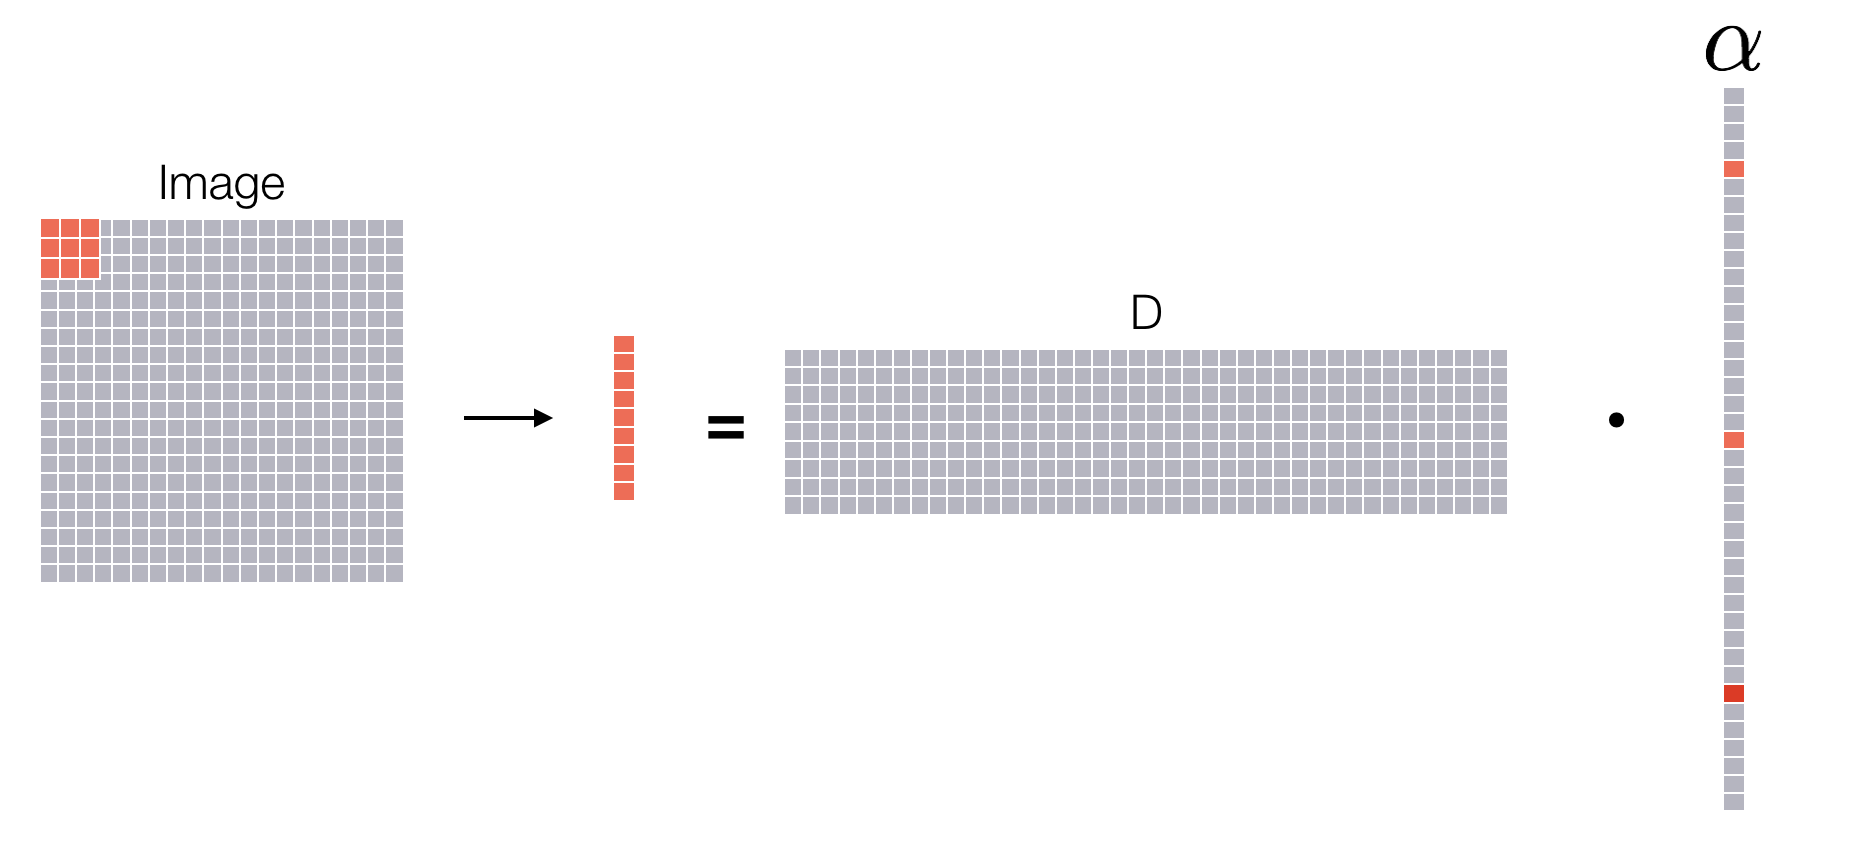
\includegraphics[width=\linewidth]{DL.png}
  \caption{sparse modeling using dictionary learning.}
\end{figure}
 Since a natural image is sparse, with the sparse modeling, we can actually represent each patch of the image in a lower dimension subspace, and remove the noise in this process.
 
 $$\mathop{\min}_{x \in R^n} ||y-D\alpha ||_2^2 \  + \lambda\ ||\alpha||_1 $$
 There are many ways to solve this problem, such as MP, or OMP. FISTA and so on. Here we use a toolbox to show some results about the performance of patch-wise sparse coding on Gaussian white noise restoration situation\cite{DBLP:journals/corr/MairalBP14}.(see footnote for more details about this toobox)
 \begin{table}[H]
 \centering
 \caption{dictionary learning performance by SPAMS toolbox}
 \begin{tabular}{ccccc}
 \toprule
  $\sigma$ & 5 & 20 & 50 & 100 \\
  \midrule
  \texttt{original Psnr}	& 34.13 & 22.16 &14.13 & 8.13   \\
   \texttt{DCT dictionary-L0 recover}	& 26.30 & 	26.60 & 23.66 & 10.12   \\
   \texttt{DCT dictionary-L1 recover}	& 25.57&	25.49 & 18.24 & 10.18  \\
   \texttt{adapted dictionary-L0 recover}	& 31.10	&30.56&	25.68&	10.34 \\
   \texttt{adapted dictionary-L1 recover}	& 32.93&	25.57&	18.79&	10.28 \\
	
  \bottomrule
 \end{tabular}
\end{table}
As data illustrated, the performance of sparse modeling is strongly related to the quality of the dictionary it is using. The parameter corresponding to $L_1$ term need to be optimized, otherwise it might not working as we expected. sometimes even achieve worse Psnr than noised image.
\footnotetext{http://spams-devel.gforge.inria.fr/doc/html/index.html}

\subsection{Convolutional Sparse Modeling}~
 As we mentioned before, A natural extension to full images instead of patches is called “convolutional sparse coding”. It consists of linearly decomposing an image by using small dictionary elements placed at all possible locations in the image. and make a circular convolution. This method replace the traditional linear representation with a sum of convolutions $\sum_{m} d_{m} * x_{m} \approx s$ where the elements of the dictionary $d_{m}$ are linear filters, and the representation consists of the set of coefficient maps $x_{m}$.\\
 	The most common form of convolutional sparse coding is Convolutional Basis Pursuit DeNoising(CBPDN), defined as
 $$ \mathrm{argmin}_\mathbf{x} \;
       (1/2) \left\| \sum_m \mathbf{d}_m * \mathbf{x}_m -
       \mathbf{s} \right\|_2^2 + \lambda \sum_m \| \alpha_m \odot \mathbf{x}_m \|_1 \eqno{(1)}$$
where the $\alpha_{m}$ allow distinct weighting of the $l_{1}$ term for each filter $d_{m}$, At present, the most efficient approach to solving this problem is via the Alternating Direction Method of Multipliers (ADMM)  framework. which solve the problem in following section:
$$\mathrm{argmin}_{\mathbf{x}, \mathbf{y}} \;
       (1/2) \left\| \sum_m \mathbf{d}_m * \mathbf{x}_m -
       \mathbf{s} \right\|_2^2 + \lambda \sum_m \| \mathbf{y}_m \|_1
       \quad \text{such that} \quad \mathbf{x}_m = \mathbf{y}_m \;\;$$
       
Solving this problem involves solving following 3 sub-problems:
\begin{flalign}
 & \mathbf{x_m}^{j+1} = \mathrm{argmin}_\mathbf{x} \;
       (1/2) \left\| \sum_m \mathbf{d}_m * \mathbf{x}_m -
       \mathbf{s} \right\|_2^2 + \rho/2 \sum_m \left\|\mathbf{x}_m -\mathbf{y}_m^j +\mathbf{u}_m \right\|_2^2 \tag{1.1}&\\  
 & \mathbf{y_m}^{j+1} = \mathrm{argmin}_\mathbf{y} \;
       \lambda \left\| \mathbf{y}_m \right\|_1 + \rho/2 \sum_m \left\|\mathbf{x}_m^{j+1} -\mathbf{y}_m +\mathbf{u}_m^j \right\|_2^2 \tag{1.2}&\\ 
&\mathbf{u}_m^{j+1} = \mathbf{u}_m^j+\mathbf{x}_m^{j+1} - \mathbf{y}_m^{j+1} \tag{1.3}& 
\end{flalign}
      where the $\mathbf{y}$ update is easily solved by applying soft thresholding like:
      $$ \mathbf{y}_l = sign\left({\mathbf{x}_m^{j+1}+ \mathbf{u}_m^{j}} \right)\odot \max{\left(0,\mathbf{x}_m^{j+1}+ \mathbf{u}_m^{j}-\lambda /\rho \right)}$$
      and $\mathbf{u}$ update is also very simple. The biggest problem is solving  $\mathbf{x}$ update, which can be solved efficiently by solving an equivalent DFT domain problem by applying Sherman–Morrison approach\cite{EGIDI2006703}.
\begin{figure}[H]
	\centering
	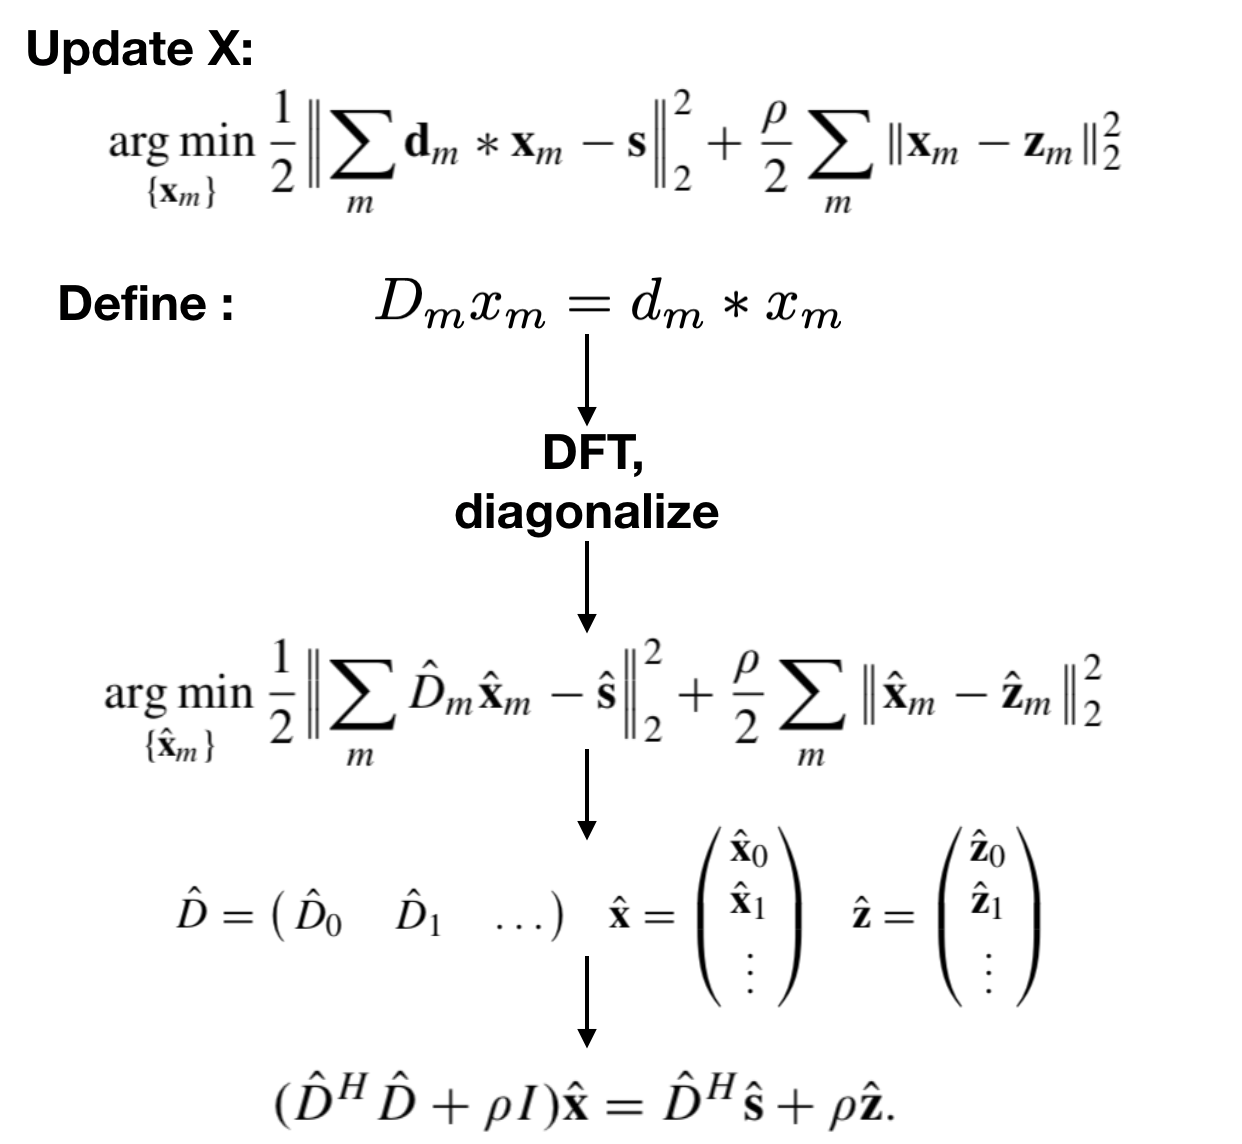
\includegraphics[scale=0.6]{X_update.png}
	\caption{structure for solving $\mathbf{x}$ sub problem }
\end{figure}
 Where $\hat{\mathbf{z}}_m =  \hat{\mathbf{y}}_m - \hat{\mathbf{u}}_m$, $\hat{D}^H\hat{D}$ has some very good structure that makes this a Diagonal Block Linear System. And can be decompose into $N$ independent $M\times M$ linear system. Each of them consists of a rank one component plus a diagonal component. and can be solved by Sherman–Morrison equality.\cite{EGIDI2006703}
 $$ \mathbf{x} = \rho^{-1}\left(\mathbf{b}-\frac{ \mathbf{a}^H \mathbf{b}}{\rho+ \mathbf{a}^H \mathbf{a}} \right)$$
In this way convolutional sparse representation can achieve many different applications efficiently. The following figure illustrate the perfirmance of CPBDN on noise restoration problem:
\begin{figure}[H]
	\centering
	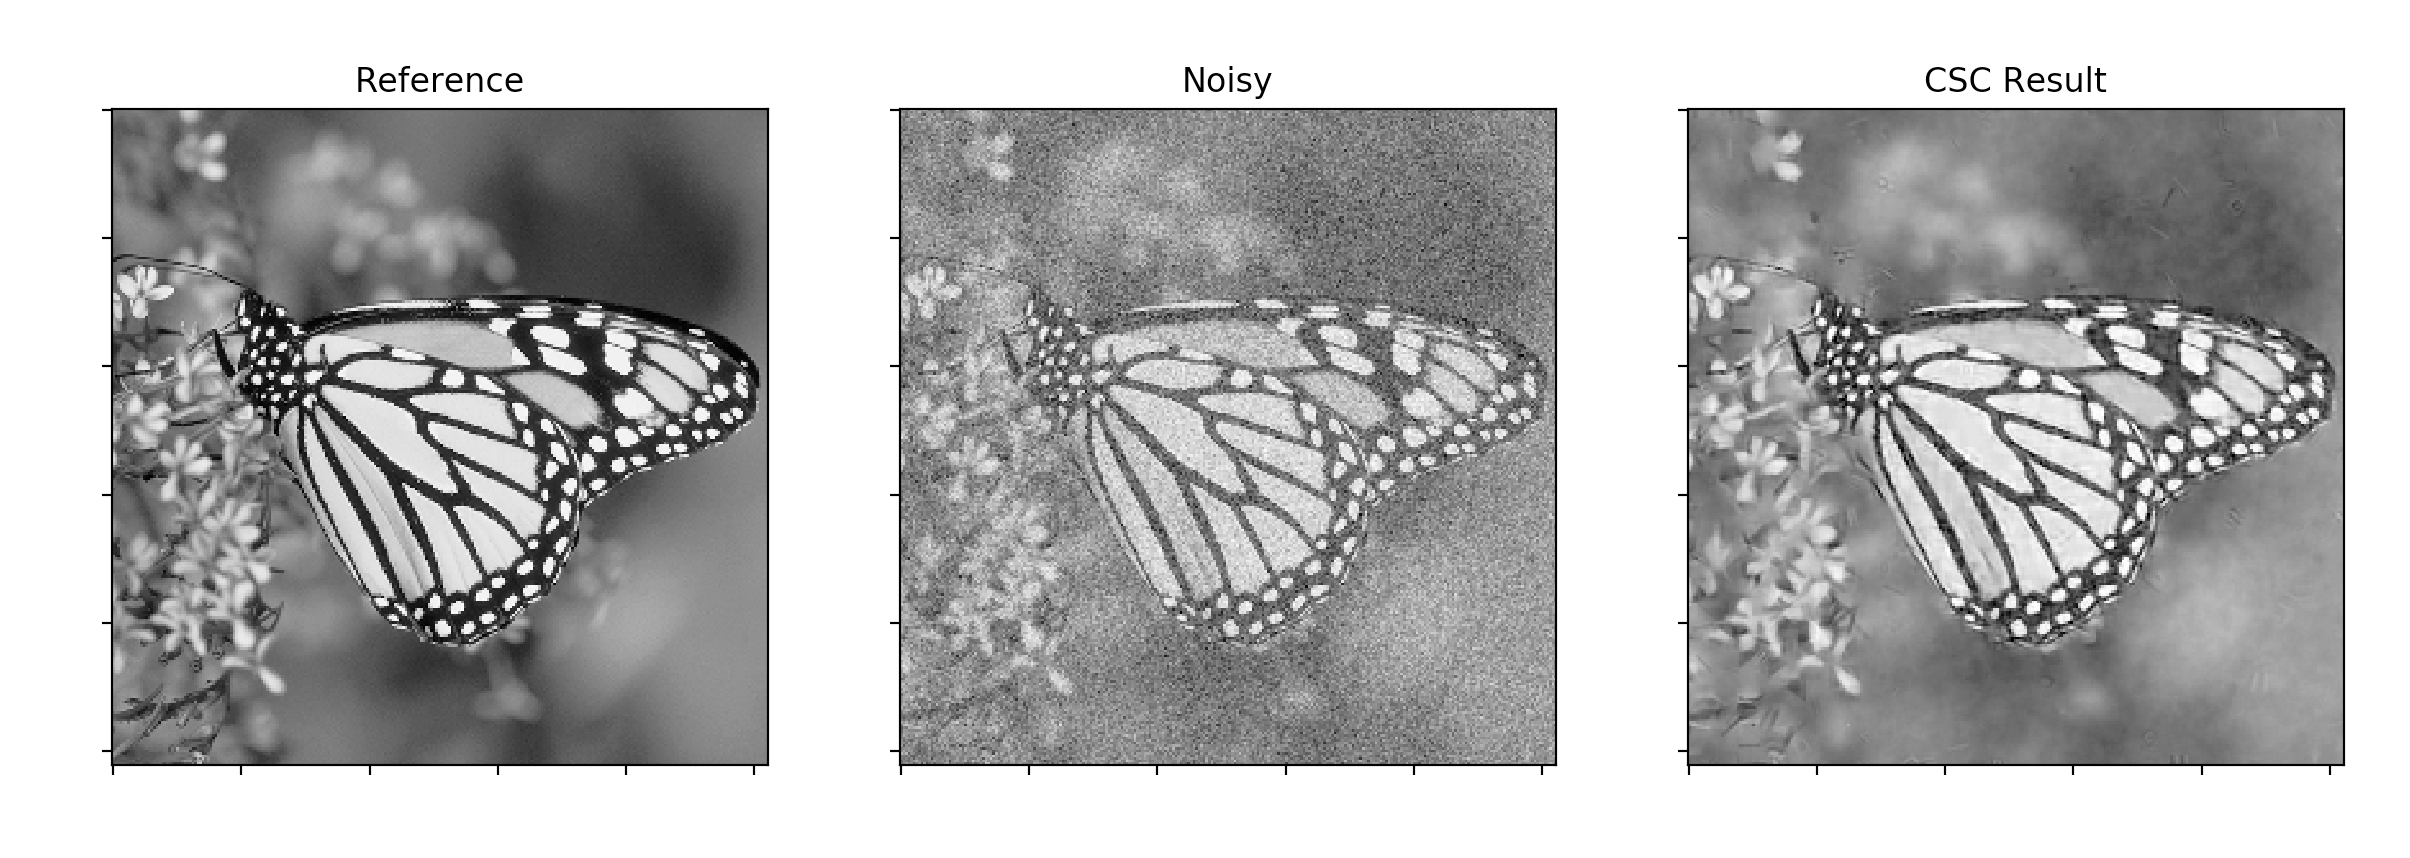
\includegraphics[width=\linewidth]{csc_recover.png}
	\caption{Convolutional sparse representation for noise removal :PSNR from 19.21 to 26.25}
\end{figure}

\section{Convolutional Sparse Coding With 2D and 3D Total Variation.}~
\subsection{Gradient Regularization}~
There is growing interest in imaging and image processing applications of the convolutional form, but they have received limited attention for image reconstruction problems. Because the convolutional sparse coding is lightly inferior to the patch-wised sparse coding in the problem of removal of the Gaussian white noise. But the performance of the convolutional form can be boosted beyond that of the patch-wised form by the inclusion of some suitable regularizations such as total variations. \\ 

An extension of (1) to include an $l_{2}$ penalty on the gradients of the coefficient maps was proposed\cite{DBLP:journals/corr/Wohlberg17a}. The primary purpose of this extension was as a regularization for an impulse filter intended to represent the low-frequency components of the image, but a small non-zero regularization on the other dictionary filters was found to provide a small improvement to the impulse noise denoising performance . Considering the edge-smoothing effect of $l_{2}$ gradient regularization, a reasonable alternative to consider is Total Variation (TV) regularization. 
It is based on the principle that signals with excessive and possibly spurious detail have high total variation, that is, the integral of the absolute gradient of the signal is high. According to this principle, reducing the total variation of the signal subject to it being a close match to the original signal.\\
\subsection{Solve of TVs on Coefficient Map}~
We consider two different variants\cite{sporco}:\\
1. scalar TV applied independently to each coefficient map:\\
$$ \mathrm{argmin}_\mathbf{x} \; \frac{1}{2}
       \left\| \sum_m \mathbf{d}_m * \mathbf{x}_m - \mathbf{s}
       \right\|_2^2 + \lambda \sum_m \| \mathbf{x}_m \|_1 +
       \mu \sum_m \left\| \sqrt{\sum_i (G_i \mathbf{x}_m)^2} \right\|_1
       \;\;$$
2.vector TV\cite{Blomgren:1998:CTT:2318958.2319497} applied jointly to the set of coefficient maps:\\
$$ \mathrm{argmin}_\mathbf{x} \; \frac{1}{2}
       \left\| \sum_m \mathbf{d}_m * \mathbf{x}_m - \mathbf{s}
       \right\|_2^2 + \lambda \sum_m \| \mathbf{x}_m \|_1 +
       \mu \left\| \sqrt{\sum_m \sum_i (G_i \mathbf{x}_m)^2} \right\|_1
       \;\;$$       
  Where $G_i$ is the gradient filter used to calculate the gradient along a specific axis of each layer of the coefficient map. We apply the same notation change shown in Figure 2, and additionally, we have:
  $$\Gamma_l = \left( \begin{array}{ccc}
          \beta_0 G_l & 0 & \ldots \\  0 & \beta_1 G_l & \ldots \\ \vdots & \vdots & \ddots
       \end{array} \right) \;\;\
 $$ 
 For l = 0 or 1, which denotes the gradient along x and y axis of each coefficient map, and for l =2, which is z axis, we have:
$$\Gamma_2 = \left( \begin{array}{ccc}
          \beta_0  & -\beta_0 & \ldots \\  0 & \beta_1  & -\beta_1 \\ \vdots & \vdots & \ddots
       \end{array} \right) \;\;$$
       Which calculate the difference between two consecutive coefficient maps.\\
       
 We solve these problem by using the same structure, For scalar TV, formally we have:
        $$
      \mathrm{argmin}_\mathbf{x} \; (1/2) \left\| D \mathbf{x} -
       \mathbf{s} \right\|_2^2 + \lambda
       \| \mathbf{x} \|_1 + \mu  \left\| \sqrt{
       (\Gamma_0\mathbf{x})^2+(\Gamma_1\mathbf{x})^2+(\Gamma_2\mathbf{x})^2} \right\|_1  \eqno{(3)} $$
  Using the same ADMM structure we can write:
  $$\mathrm{argmin}_\mathbf{x} \; (1/2) \left\| D \mathbf{x} -
       \mathbf{s} \right\|_2^2 + \lambda
       \| \mathbf{y}_L \|_1 + \mu \sum_m \left\| \sqrt{
       \mathbf{y}_0^2+\mathbf{y}_1^2+\mathbf{y}_2^2} \right\|_1 \quad $$
       $$ \text{ s.t. } \quad
       \left( \begin{array}{c} \Gamma_0 \\ \Gamma_1 \\ \Gamma_2 \\ I
       \end{array} \right) \mathbf{x} =
       \left( \begin{array}{c} \mathbf{y}_0 \\
       \mathbf{y}_1 \\ \mathbf{y}_2 \\ \mathbf{y}_3 \end{array}
       \right)  \;\; \eqno{(4)}$$
       The resulting $\mathbf{x}$ sub-problem has the form:
       $$\mathrm{argmin}_{\mathbf{x}} \; 1/2\left\| D\mathbf{x} - \mathbf{s}\right\|_2^2 + (\rho/2)\left\| \Gamma_0\mathbf{x} -
       \mathbf{y}_0 +\mathbf{u}_0\right\|_2^2 +(\rho/2)\left\| \Gamma_1\mathbf{x} -
       \mathbf{y}_1 +\mathbf{u}_1\right\|_2^2 $$
       $$+(\rho/2)\left\| \Gamma_2\mathbf{x} -
       \mathbf{y}_2 +\mathbf{u}_2\right\|_2^2 +(\rho/2)\left\| \mathbf{x} -
       \mathbf{y}_3 +\mathbf{u}_3 \right\|_2^2 \eqno{(4.1)} $$
       And the solution of the equivalent DFT domain problem is given by:
       $$
     \left(  \hat{D}^H\hat{D}+\rho I +\rho\hat{\Gamma_0}^H\hat{\Gamma_0}+\rho\hat{\Gamma_1}^H\hat{\Gamma_1}+\rho\hat{\Gamma_2}^H\hat{\Gamma_2}\right)\hat{\mathbf{x}}=
$$
$$
\hat{D}^H \hat{s} + \rho\left( \hat{y}_3-\hat{u}_3+
\hat{\Gamma}_0^H\left(\hat{y}_0-\hat{u}_0\right)+
\hat{\Gamma}_1^H\left(\hat{y}_1-\hat{u}_1\right)+
\hat{\Gamma}_2^H\left(\hat{y}_2-\hat{u}_2\right)
\right)
$$
Since all $\hat{\Gamma}_l^H\hat{\Gamma}$ are diagonal (the $\hat{G}_i$ are diagonal, and therefore so are $\hat{\Gamma}_i$), they can be grouped together with the $\rho I$ term; The system is again a Diagonal Block Linear System and the Sherman-Morrison solution\cite{EGIDI2006703} can be directly applied without any substantial increase in computational cost.\\
The $\mathbf{y}$ sub-problem for $(4)$ can be decomposed into the independent problems.
$$\mathrm{argmin}_{\mathbf{y_3}} \; \rho/2 \| \mathbf{x} -\mathbf{y}_3+\mathbf{u}_3\|_2^2 + \lambda\| \mathbf{\alpha \odot \mathbf{y_3}}\| \eqno{(4.2.1)}
$$
$$
\mathrm{argmin}_{\mathbf{y_0},\mathbf{y_1},\mathbf{y_2}} \; \mu \| \mathbf{y}_0^2 +\mathbf{y}_1^2+\mathbf{y}_2^2\|_1 + (\rho/2)\left\| \mathbf{x} -
       \mathbf{y}_0 +\mathbf{u}_0\right\|_2^2 +$$
       $$(\rho/2)\left\| \mathbf{x} -
       \mathbf{y}_1 +\mathbf{u}_1\right\|_2^2 +(\rho/2)\left\| \mathbf{x} -
       \mathbf{y}_2 +\mathbf{u}_2\right\|_2^2 \eqno{(4.2.2)}
       $$
       The solution to $(4.2.1)$ is the same as y update for traditional convolutional sparse representation, and $(4.2.2)$ can be solved by use of the block soft thresholding operation applied in the same way as in the ADMM algorithm for the standard isotropic TV denoising problem like:
       $$\mathbf{y}_l = \frac{\mathbf{z}_l}{\sqrt{\mathbf{z}_0^2+\mathbf{z}_1^2+\mathbf{z}_2^2}}\max{\left(0,\sqrt{\mathbf{z}_0^2+\mathbf{z}_1^2+\mathbf{z}_2^2}-\frac{\mu}{\rho}\right)}$$ 
       For 2D TV, simply remove all the $y_2$ and $\Gamma_2$ part inside each equation. For vector TV, we can treat the set of coefficient maps as a multi-channel image and apply Vector TV\cite{Blomgren:1998:CTT:2318958.2319497}. There is only small differences between this algorithm and scalar TV, see\cite{DBLP:journals/corr/Wohlberg17a} for more details.
 \subsection{Experiments Setup and Results}~
 In order to compare the performance of different kinds of TV regularizer, We designed following experiments. The experiments of different TV as well as traditional patch-wise and convolutional sparse coding is conduct on Gaussian white noise restoration problem on 128 by 128 grey scale Barbara image\cite{7532675} with noise's standard deviation 0.1. For convolutional sparse representation I'm using a fixed convolutional dictionary of size 8*8*14 given by Sporco library. While the  patch-wise dictionary  consisted of 32 vectors of 64 coefficients each(i.e a vectorized 8 by 8 image block).The CBPDN decomposition was applied to highpass filtered images, obtained by subtracting a lowpass component computed by Tikhonov regularization. For each situation parameters has been optimized manually.\\ 
 
 Here is the wrap up result graph I have:
\begin{figure}[H]
  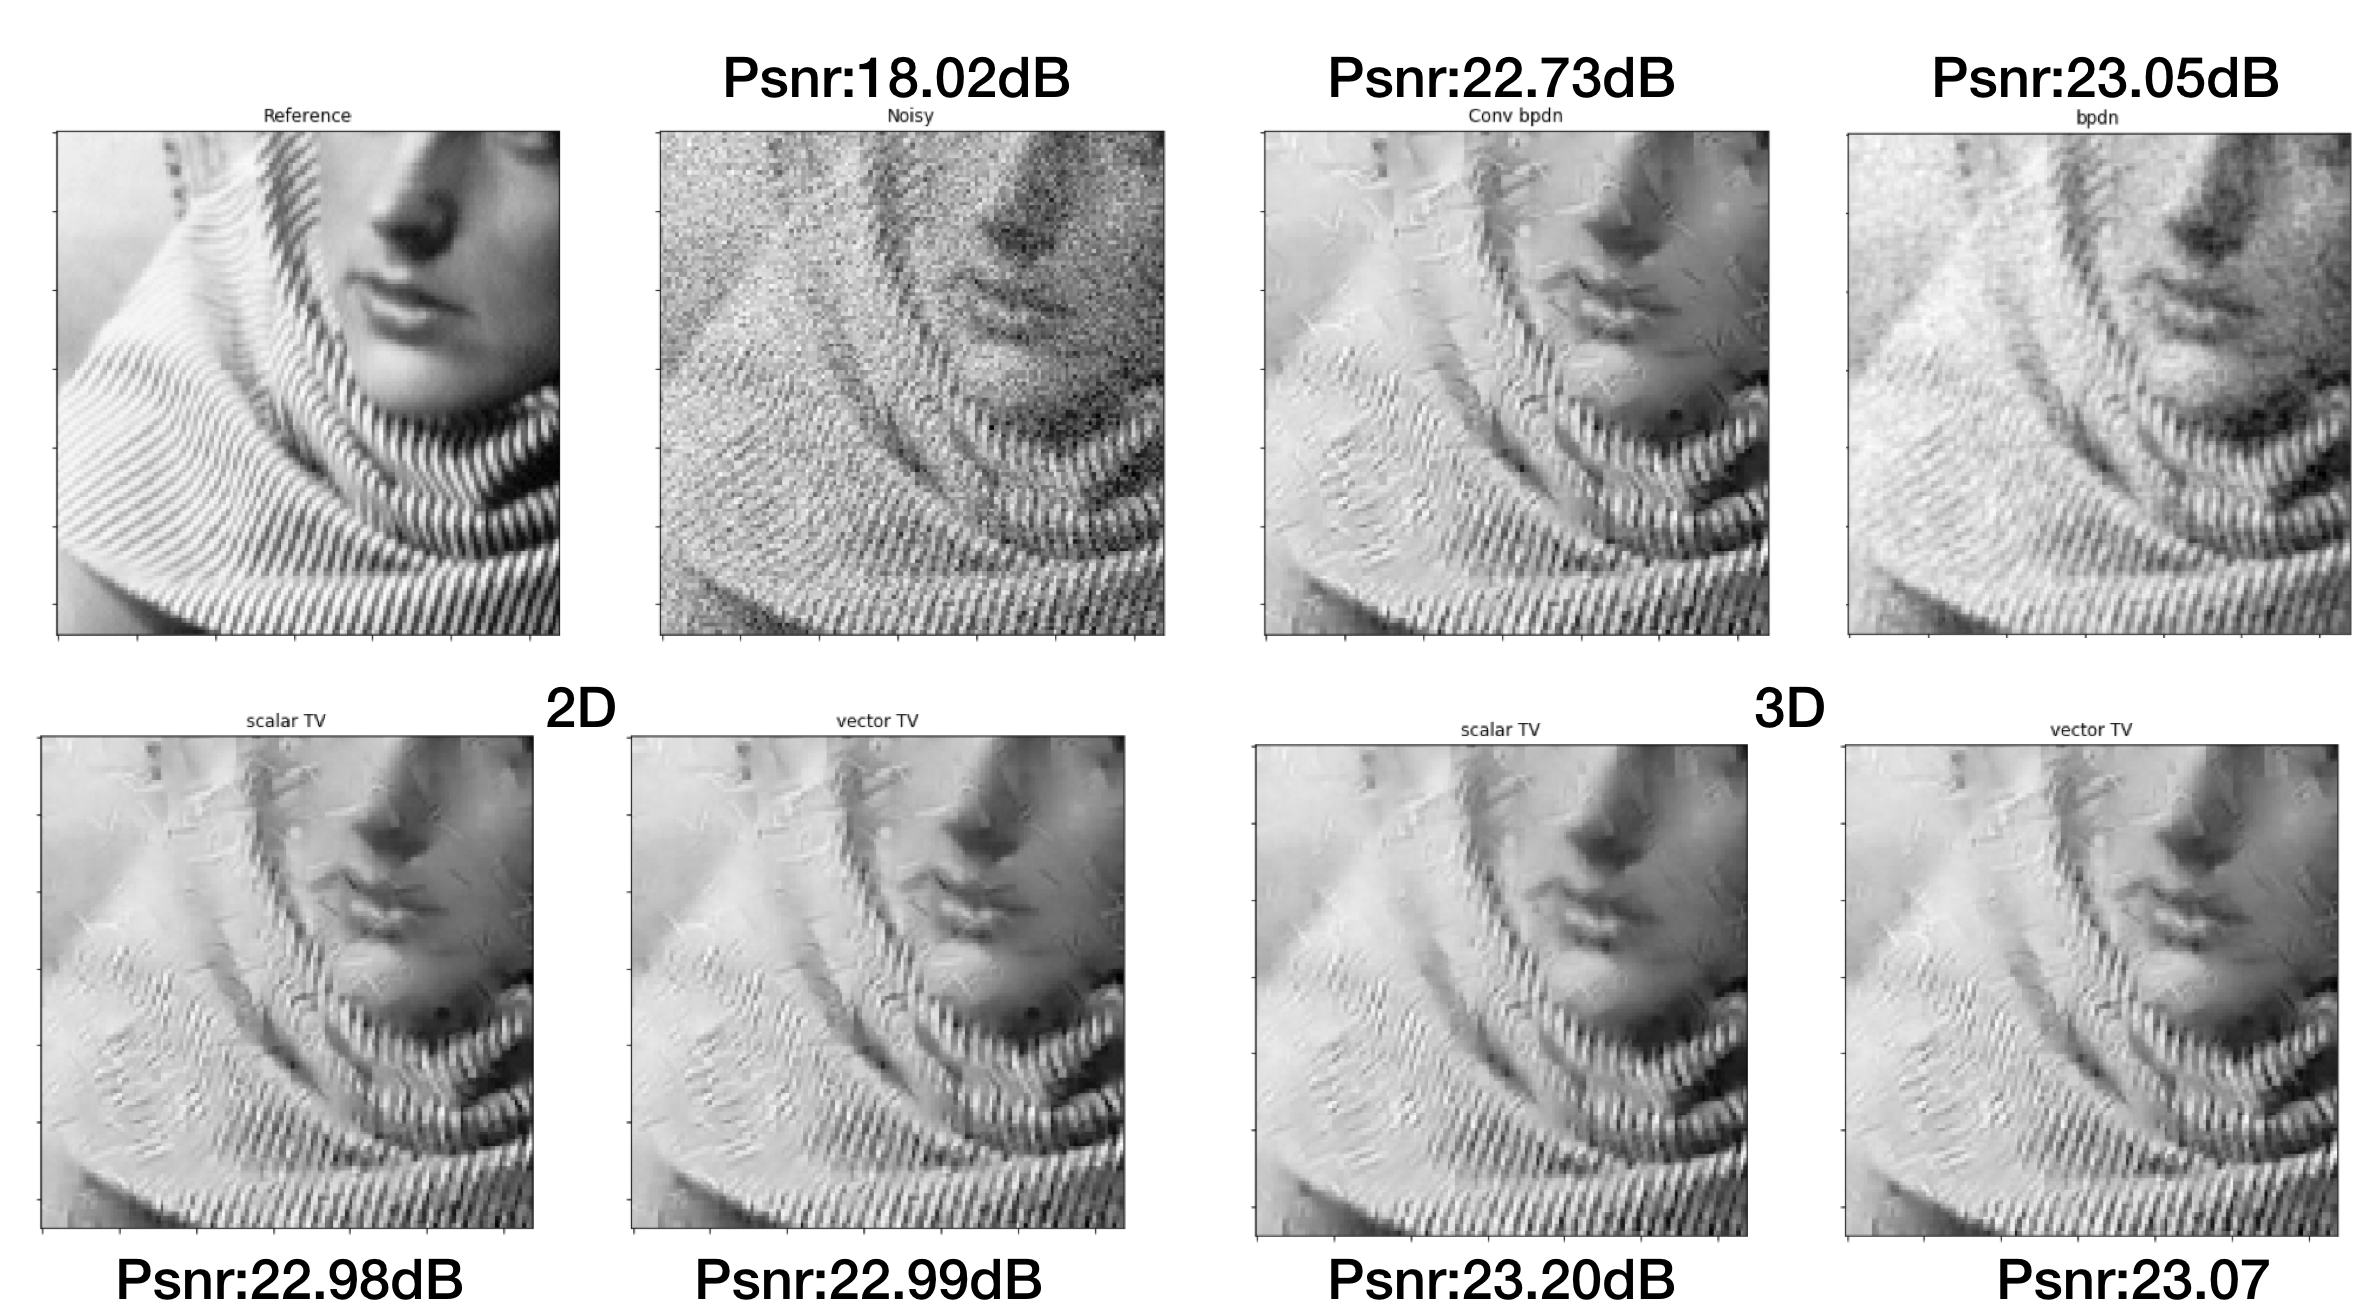
\includegraphics[width=\linewidth]{8_result.png}
  \caption{Result of convolutional sparse coding with different TV \cite{sporco}}
\end{figure}

To clearify: From the top left to right we have: original image, the noisy image, denoised image by convolutional sparse representation, denoised image by patch-wise sparse representation. From the bottom left to right we have: denoised image by 2D scalar TV and convolutional sparse representation, denoised image by 2D vector TV and convolutional sparse representation, denoised image by 3D scalar TV and convolutional sparse representation, denoised image by 3D vector TV and convolutional sparse representation.\\

We also test the differences of performance between 2D and 3D scalar TV corresponding to the number of dictionary layers, The graph below illustrate how psnr of 2D scalar TV and 3D scalar TV change with respect to the number of dictionary layers. Number of layers is from 1 to 14. Note that psnr is not linearly increasing as the number of layers increases, One possible assumption is that those layers doesn't include necessary features or patterns for representing this image.
\begin{figure}[H]
  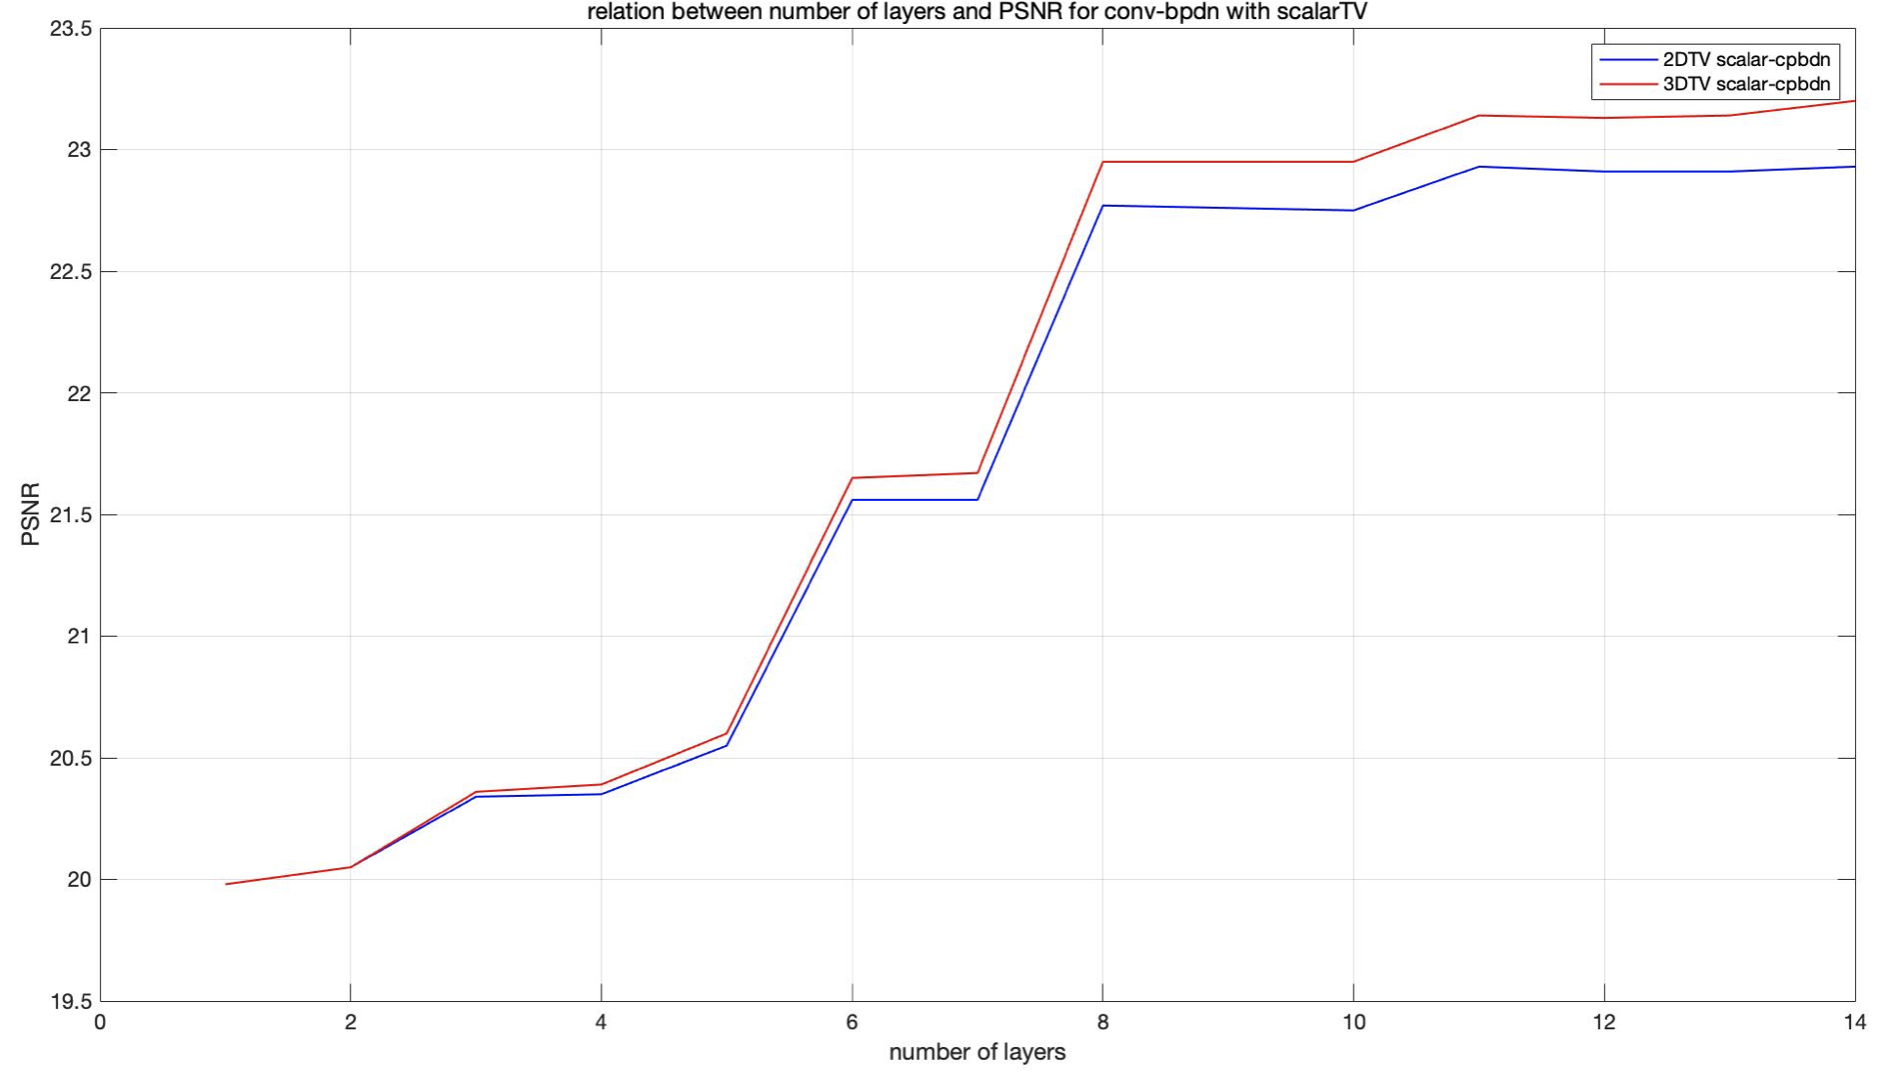
\includegraphics[width=\linewidth]{layer_psnr.png}
  \caption{Relation between psnr and number of dictionary layers }
\end{figure}\section{Conclusions and Future Work}~


The performance of sparse representation is strongly connected to the quality and the size of dictionary, and convolutional dictionary is quite different from the traditional dictionary(more layers) so a strictly apples-to-apples comparison between BPDN and CBPDN denoising methods is difficult to construct, the careful attempt reported here indicates that BPDN is slightly superior to baseline CBPDN, but that augmentation of the baseline CBPDN functional with the appropriate TV term substantially boosts performance. With respect to the specific form of additional TV term, scalar TV applied independently to each coefficient map is somewhat superior to a joint vector TV term over all of the coefficient maps, furthermore, both 3D scalar TV and vector TV achieves better performance than it's 2D version,This difference becomes more apparent as the number of layers increases.In my experiments 3D scalar TV performance even better than patch-wise sparse representation.\\

However, We need more experiments to confirm this conclusion.the results we have now suggest that penalties that exploit the spatial structure, especially the structure between each layers of the coefficients are necessary to achieve the true potential of the convolutional model.\cite{DBLP:journals/corr/Wohlberg17a}


 
\section{Acknowledgements}~


I'd like to thank everyone in this Lab for their kindness and help, Thanks to Prof.Kamilov for everything he taught to me and giving me this project idea and guidance throughout my work,Thanks to Yu Sun's advice about the schedule and how to start my work. Special thanks to XiaoJian and JiaLong for helping me debug my code and lots of advise during my implementation.
 

\newpage


\bibliographystyle{IEEEbib}
\bibliography{refs}
  


\end{document}
